\section{Validierung}
Dieses Kapitel stellt das Ergebnis dieser Arbeit vor. Weiterhin werden die in 
Kapitel~\ref{sec:fas} und~\ref{sec:nfas} definierten Anforderungen verifiziert.

\subsection{Ergebnis}
Das Projekt ``TestHub'' konnte erfolgreich umgesetzt und die in Abschnitt~\ref{sec:problems}
definierten Probleme somit umfassend gelöst werden. 
In den folgenden Abbildungen kann die finale Version des Projekts angesehen werden.
Da das Projekt nur firmenintern nutzbar ist, wurde ein Video 
(\textit{videos/abchlussdemo.mp4}) erstellt, welches alle Funktionen des 
Projekts aufzeigt. 

\begin{figure}[H]
    \includegraphics[width=\linewidth]{img/DashboardFinal.png}
    \caption{Das finale Dashboard}
\end{figure}

\begin{figure}[H]
    \includegraphics[width=\linewidth]{img/SucheFinal.png}
    \caption{Die Suchansicht mit jedem Equipment nach Kategorie sortiert}
\end{figure}

\begin{figure}[H]
    \includegraphics[width=\linewidth]{img/RessourceFinal.png}
    \caption{Die Detailansicht einer Ressource}
\end{figure}

\subsection{Verifizierung der Anforderungen}



\subsection{Validierung der Bedienbarkeit}
Um die Bedienbarkeit von TestHub zu analysieren, wird der in Abschnitt~\ref{sec:problems}
angeführt alte Prozess mit dem neuen durch TestHub optimierten Prozess verglichen.
Folgende Aufgaben werden ausgeführt:

\begin{enumerate}
    \item Heraussuchen des Jira Tickets, welches auf das Ticket C3003889-2681 folgt.
    \item Heraussuchen der Ressourcen, welche in den nächsten 30 Tagen gewartet werden sollen.
    \item Einer Ressource einen neuen Wartungstermin hinzufügen und diesen mit dem Team synchronisieren.
\end{enumerate}

Um aussagekräftige Daten zu erhalten, wird neben der Zeit auch die Cursordistanz,
die Mausradticks und Klickzahl gemessen. Zu diesem Zweck wurde das Programm OdoPlus\footurl{https://www.fridgesoft.de/odoplus.php}
verwendet.

\begin{figure}[H]
    \centering
    \begin{subfigure}{.5\textwidth}
      \centering
      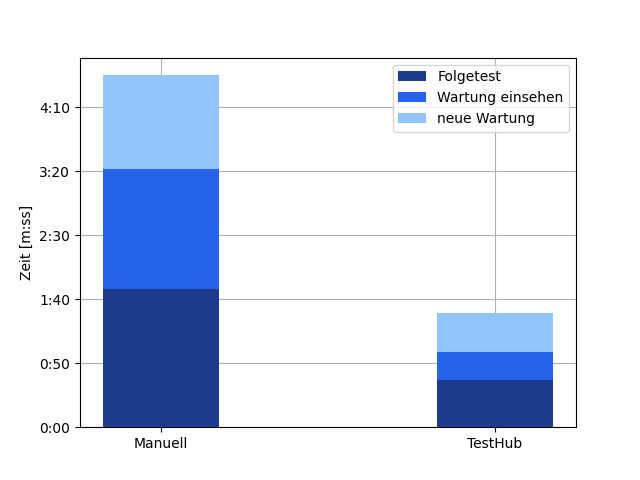
\includegraphics[width=\linewidth]{speedtests/validierung_Zeit.png}
      \caption{Zeitersparnis}
    \end{subfigure}%
    \begin{subfigure}{.5\textwidth}
      \centering
      \includegraphics[width=\linewidth]{speedtests/validierung_cursordistanz.png}
      \caption{Mauszeigerdistanz}
    \end{subfigure}\\
    \begin{subfigure}{.5\textwidth}
        \centering
        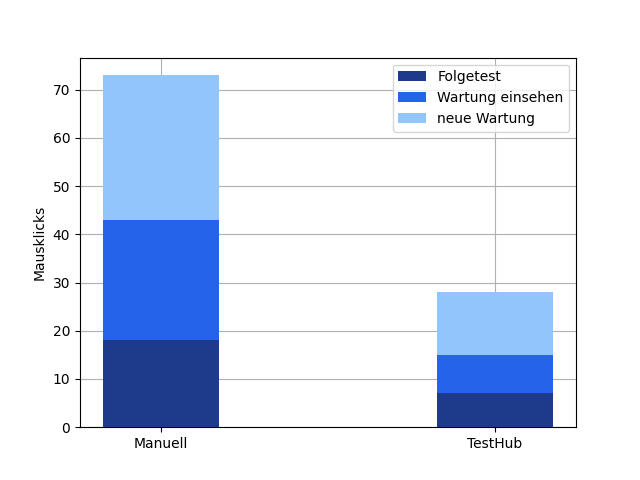
\includegraphics[width=\linewidth]{speedtests/validierung_Mausklicks.png}
        \caption{Mausklicks}
      \end{subfigure}%
      \begin{subfigure}{.5\textwidth}
        \centering
        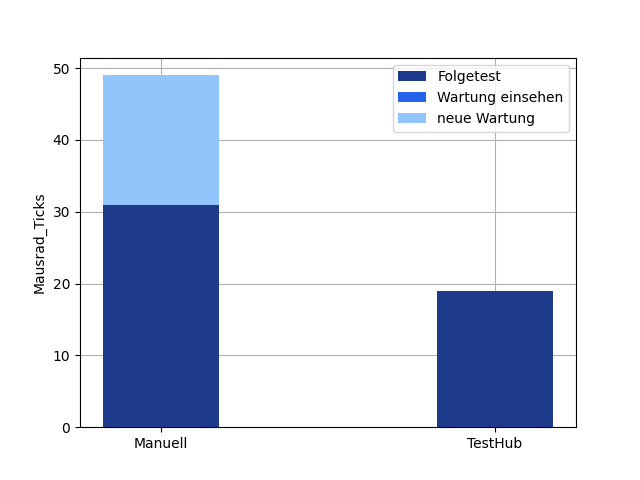
\includegraphics[width=\linewidth]{speedtests/validierung_Mausrad_Ticks.png}
        \caption{Mausrad Ticks}
      \end{subfigure}
    \caption{Ergebnisse der Bedienbarkeitsvalidierung, aufgeschlüsselt nach Aufgaben}
\end{figure}

Auf den ersten subjektiven Blick fällt auf, dass TestHub in fast allen Bereichen eine 
Verbesserung von groben 50\% aufweist. Gerade der wichtigste Faktor, der Zeitaufwand, ist durch TestHub 
erheblich geringer. Nur bei der Erstellung eines neuen Wartungstermins
ist die Mauszeigerdistanz etwas größer als bisher, da in einem maximierten Browserfenster
gearbeitet wird statt im kleinen Windows Dateiexplorer Fenster. Auch auffallend ist,
dass nur beim Folgetest heraussuchen das Mausrad benutzt werden muss. Die Benutzung des 
Mausrads beim erstellen eines neuen Wartungstermins fällt komplett weg, was für 
eine Übersichtlichkeit des Designs spricht.

Um diese Aussagen zu belegen, müsste jedoch eine viel größere Studie mit mehreren 
Teilnehmern und Testfällen durchgeführt werden.



